
\documentclass[12pt]{article}

\usepackage{fancyhdr} % Required for custom headers
\usepackage{lastpage} % Required to determine the last page for the footer
\usepackage{extramarks} % Required for headers and footers
\usepackage{graphicx} % Required to insert images
\usepackage{amsmath}
\usepackage{float}
\usepackage{bm}
\usepackage{listings}
%\usepackage{lipsum} % Used for inserting dummy 'Lorem ipsum' text into the template
% Margins
\topmargin=-0.45in
\evensidemargin=0in
\oddsidemargin=0in
\textwidth=6.5in
\textheight=9.0in
\headsep=0.25in 
\linespread{1.1} % Line spacing
% Set up the header and footer
\pagestyle{fancy}
\lhead{\hmwkAuthorName} % Top left header
\chead{\hmwkClass\ : \hmwkTitle} % Top center header
\rhead{\firstxmark} % Top right header
\lfoot{\lastxmark} % Bottom left footer
\cfoot{} % Bottom center footer
\rfoot{Page\ \thepage\ of\ \pageref{LastPage}} % Bottom right footer
\renewcommand\headrulewidth{0.4pt} % Size of the header rule
\renewcommand\footrulewidth{0.4pt} % Size of the footer rule
\setlength\parindent{0pt} % Removes all indentation from paragraphs

%----------------------------------------------------------------------------------------
%	DOCUMENT STRUCTURE COMMANDS
%----------------------------------------------------------------------------------------

% Header and footer for when a page split occurs within a problem environment
\newcommand{\enterProblemHeader}[1]{
\nobreak\extramarks{#1}{#1 continued on next page\ldots}\nobreak
\nobreak\extramarks{#1 (continued)}{#1 continued on next page\ldots}\nobreak
}

% Header and footer for when a page split occurs between problem environments
\newcommand{\exitProblemHeader}[1]{
\nobreak\extramarks{#1 (continued)}{#1 continued on next page\ldots}\nobreak
\nobreak\extramarks{#1}{}\nobreak
}

\setcounter{secnumdepth}{0} % Removes default section numbers
\newcounter{homeworkProblemCounter} % Creates a counter to keep track of the number of problems

\newcommand{\homeworkProblemName}{}
\newenvironment{homeworkProblem}[1][Problem \arabic{homeworkProblemCounter}]{ % Makes a new environment called homeworkProblem which takes 1 argument (custom name) but the default is "Problem #"
\stepcounter{homeworkProblemCounter} % Increase counter for number of problems
\renewcommand{\homeworkProblemName}{#1} % Assign \homeworkProblemName the name of the problem
\section{\homeworkProblemName} % Make a section in the document with the custom problem count
\enterProblemHeader{\homeworkProblemName} % Header and footer within the environment
}{
\exitProblemHeader{\homeworkProblemName} % Header and footer after the environment
}

\newcommand{\problemAnswer}[1]{ % Defines the problem answer command with the content as the only argument
\noindent\framebox[\columnwidth][c]{\begin{minipage}{0.98\columnwidth}#1\end{minipage}} % Makes the box around the problem answer and puts the content inside
}

\newcommand{\homeworkSectionName}{}
\newenvironment{homeworkSection}[1]{ % New environment for sections within homework problems, takes 1 argument - the name of the section
\renewcommand{\homeworkSectionName}{#1} % Assign \homeworkSectionName to the name of the section from the environment argument
\subsection{\homeworkSectionName} % Make a subsection with the custom name of the subsection
\enterProblemHeader{\homeworkProblemName\ [\homeworkSectionName]} % Header and footer within the environment
}{
\enterProblemHeader{\homeworkProblemName} % Header and footer after the environment
}
   
%----------------------------------------------------------------------------------------
%	NAME AND CLASS SECTION
%----------------------------------------------------------------------------------------

\newcommand{\hmwkTitle}{Homework 5} % Assignment title
\newcommand{\hmwkDueDate}{\date} % Due date
\newcommand{\hmwkClass}{STAT\ 580} % Course/class
\newcommand{\hmwkAuthorName}{Haozhe Zhang} % Your name

%----------------------------------------------------------------------------------------

\begin{document}


	\begin{homeworkProblem}
		\noindent \textbf{(a)}
		
		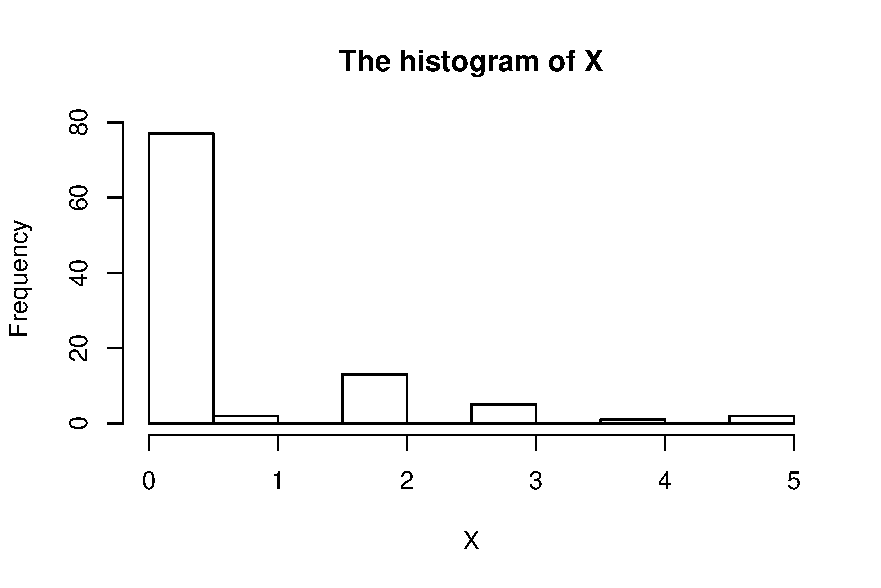
\includegraphics[width=0.8\linewidth]{HW5_1_a.pdf}
		\lstinputlisting[language=R]{../hw5_1_a.R}
		
		\noindent \textbf{(b)}
		\begin{eqnarray*}
		f(\lambda|p,\bm{r},\bm{x}) &\propto& \lambda^{a-1+\sum_{i=1}^{n}x_{i}}\exp(-b\lambda+\lambda\sum_{i=1}^{n}x_{i})\\
		f(p|\lambda,\bm{r},\bm{x}) &\propto& p^{\sum_{i=1}{n}r_{i}}(1-p)^{n-\sum_{i=1}{n}r_{i}}\\
		f(r_{i}|\lambda,p,\bm{x}) &\propto& \left(e^{-\lambda}\frac{p}{1-p}\right)^{r_{i}}r_{i}^{x_{i}}\\
		\end{eqnarray*}\\
		
		\noindent \textbf{(c)}
		\begin{itemize}
			\item For $a=1$ and $b=1$, the $95\%$ confidence interval of $\lambda$ is $ (1.511976, 2.824471 )$, and the $95\%$ confidence interval of $p$ is $ (0.1802548, 0.3769580  )$.
			\item For $a=1$ and $b=10$, the $95\%$ confidence interval of $\lambda$ is $ (1.013360, 1.918225)$, and the $95\%$ confidence interval of $p$ is $ (0.2049541, 0.4450217 )$.
			\item For $a=10$ and $b=1$, the $95\%$ confidence interval of $\lambda$ is $ (1.921057, 3.296289)$, and the $95\%$ confidence interval of $p$ is $ (0.1799374, 0.3731253 )$.
			\item For $a=10$ and $b=10$, the $95\%$ confidence interval of $\lambda$ is $ (1.306673, 2.288253)$, and the $95\%$ confidence interval of $p$ is $ (0.1927605, 0.3973745 )$.
		\end{itemize}
		\lstinputlisting[language=R]{../hw5_1_c.R}
	\end{homeworkProblem}


\begin{homeworkProblem}
\begin{itemize}
	\item For $Gamma(1,1)$, the absolute error of $E(Z)$ is $ 0.0106$ and the absolute error of $E(1/Z)$ is $0.0081$.
		\item For $Gamma(1,10)$, the absolute error of $E(Z)$ is $ 0.2968$ and the absolute error of $E(1/Z)$ is $0.1942$.
			\item For $Gamma(10,1)$, the absolute error of $E(Z)$ is $ 0.4547$ and the absolute error of $E(1/Z)$ is $0.3125$.
				\item For $Gamma(10,10)$, the absolute error of $E(Z)$ is $ 0.0289$ and the absolute error of $E(1/Z)$ is $0.0117$.
				\item For $Gamma(0.1,0.1)$, the absolute error of $E(Z)$ is $ 0.0096$ and the absolute error of $E(1/Z)$ is $0.0134$.
\end{itemize}
	\noindent \textbf{R code:}
	\lstinputlisting[language=R]{../hw5_2.R}
\end{homeworkProblem}


\begin{homeworkProblem}

	\noindent \textbf{C code:}
	\lstinputlisting[language=C]{../hw5_3.c}
\end{homeworkProblem}

\end{document}
